

%% NOVAC
%% =============
%%
This chapter outlines the algorithm which is used for the evaluation of the spectroscopic data recorded in NOVAC. 
The problem of contamination of the reference is explained and possible solutions are presented.

\section{Conventional evaluation routine}
The fitting routine used for this thesis is based on the DOASIS software \citep{kraus2006doasis}. 
The equations of the DOAS retrieval of this work are slightly different from \Cref{eq:taustrich} and therefore described in the following.
\Cref{eq:lbe} can be rewritten as:
\begin{align}
ln\left(I\left(\lambda, L\right)\right) = &ln\left(I_0 \right) + P \left(\lambda\right) -	\int_{0}^{L}\sum_{j}\sigma_j \left(\lambda, p, T \right) \cdot c_j \left(l\right)dl \nonumber \\
= &ln\left(I_0 \right) + P \left(\lambda\right)-
\sum_{j}\sigma_j \left(\lambda, p, T \right) \cdot S_j
\label{eq:lben}
\end{align}
%
The polynomial $ P \left(\lambda\right)$ accounts for all broad-band effects which approximates the scattering effects of the atmosphere as well as broad band absorptions.

The task of the DOAS retrieval is to find a model function $F \left(\lambda\right)$ that minimizes $\chi^2$:
\begin{equation}
\chi^2 = \sum_{i=\lambda_1}^{\lambda_2}\left(ln(I(i))-F(i)\right)^2
\label{eq:Chi}
\end{equation}
While $F\left(\lambda\right)$ can be expressed on the basis of \Cref{eq:lben}:
\begin{equation}
F\left(\lambda\right) = ln\left(I_0 \right) + P \left(\lambda\right)-
\sum_{j}\sigma_j \left(\lambda\right) \cdot S_j
\label{eq:F}
\end{equation}
The DOAS fitting routine uses a combination of a standard least-squares fit and a Levenberg-Marquard algorithm to minimize $\chi^2$\\
\\
Prior to the DOAS fitting. the spectra need to be calibrated, this done by using a wavelength to pixel mapping function (WMP) developed by \citet{lehman 2014}. The WMP uses a solar atlas spectrum that is concolced with the Hg line of the single instruments, hereby am initial calibration based on the Hg lines is given as a first parameter. The calibration is done by fitting the Fraunhofer lines of the recorded spectrum on the convolved Solar Atlas spectrum. The Rayleigh scattering is considered by adding a Ring spectrum as well as a wavelength dependent Ring spectrum (proportional to $\lambda^4$) \citep{wagner2009}. Mie scattering and broadband absorption structures were accounted due to adding a third order polynomial to the retrieval well as an offset polynomial to correct for stray-light influence \citep{lubcke2014bro}.\\
The \ce{SO2} evaluation is performed for a wavelength range between 314.8~nm and 328~nm. Including a \ce{SO2} absorption cross section recorded at a temperature of 298K \citep{vandaele2009fourier} and a  \ce{O3} absorption cross section recorded at 221K \citep{burrows1999atmospheric}.\\
The \ce{BrO}  evaluation is performed for a wavelength range between 330.6~nm and 352.7~nm (found by \citet{vogel2011volcanic}). The sum in \Cref{eq:F} includes for the BrO evaluation the following absorption cross sections:
\ce{BrO}  at 298K \citep{fleischmann2004new}, the \ce{SO2} and  \ce{O3} absorption cross sections described above, \ce{O4} \citep{hermans2003absorption},  \ce{NO2} at 298K \citep{vandaele1998measurements} and  \ce{CH2O} at 298K \citep{meller2000temperature}.\\
%
The choice of the wavelength range as well as the considered trace gases used in the fits is based on studies on the optimal evaluation wavelength range in a combination of real measurement data and theoretical studies 
Prior to the DOAS fitting. the spectra need to be calibrated, this done by using a wavelength to pixel mapping function (WMP) developed by \citet{lehman 2014}. The WMP uses a solar atlas spectrum that is concolced with the Hg line of the single instruments, hereby am initial calibration based on the Hg lines is given as a first parameter. The calibration is done by fitting the Fraunhofer lines of the recorded spectrum on the convolved Solar Atlas spectrum. The Rayleigh scattering is considered by adding a Ring spectrum as well as a wavelength dependent Ring spectrum (proportional to $\lambda^4$) \citep{wagner2009}. Mie scattering and broadband absorption structures were accounted due to adding a third order polynomial to the retrieval well as an offset polynomial to correct for stray-light influence \citep{lubcke2014bro}.\\
The \ce{SO2} evaluation is performed for a wavelength range between 314.8~nm and 328~nm. Including a \ce{SO2} absorption cross section recorded at a temperature of 298K \citep{vandaele2009fourier} and a  \ce{O3} absorption cross section recorded at 221K \citep{burrows1999atmospheric}.\\
The \ce{BrO}  evaluation is performed for a wavelength range between 330.6~nm and 352.7~nm (found by \citet{vogel2011volcanic}). The sum in \Cref{eq:F} includes for the BrO evaluation the following absorption cross sections:
\ce{BrO}  at 298K \citep{fleischmann2004new}, the \ce{SO2} and  \ce{O3} absorption cross sections described above, \ce{O4} \citep{hermans2003absorption},  \ce{NO2} at 298K \citep{vandaele1998measurements} and  \ce{CH2O} at 298K \citep{meller2000temperature}.\\
%
The choice of the wavelength range as well as the considered tracfor BrO and SO2, made by \citet{vogel2011volcanic}.\\
The spectra of the trace gases were convoluted by using the 334.15 nm line of a mercury lamp.\\
A further effect influencing the evaluation is the $I_{0}$ effect, in order to account for the I0-effect \citep{platt2008differential} an
iterative approach was used. Further informations can be found at (Wagner et al., 2002), \cite{lubcke2014bro},\cite{vogel2011volcanic}).
To further correct for small inaccuracies of the WMP, the FRS and both Ring spectra as one set, and all trace gases absorption cross sections as another set, are allowed to be shifted, and first order squeezed against the measurement spectrum.\\
%
NOVAC provides spectral data for roughly 50 different elevation angles. For the DOAS evaluation a reference and a measurement spectrum is needed. Obtaining the complete amount of volcanic gases is only possible in the case of the availability of references which are free of volcanic gases of interest(this will be discussed more detailed in \Cref{Chap:Cont}). The column density of  \ce{BrO}  and \ce{SO2} of the measurement spectrum relatively to the reference spectrum can be calculated \Cref{eq:Chi} and \ref{eq:F}. \\
\\
\begin{figure}
	\subfigure[]{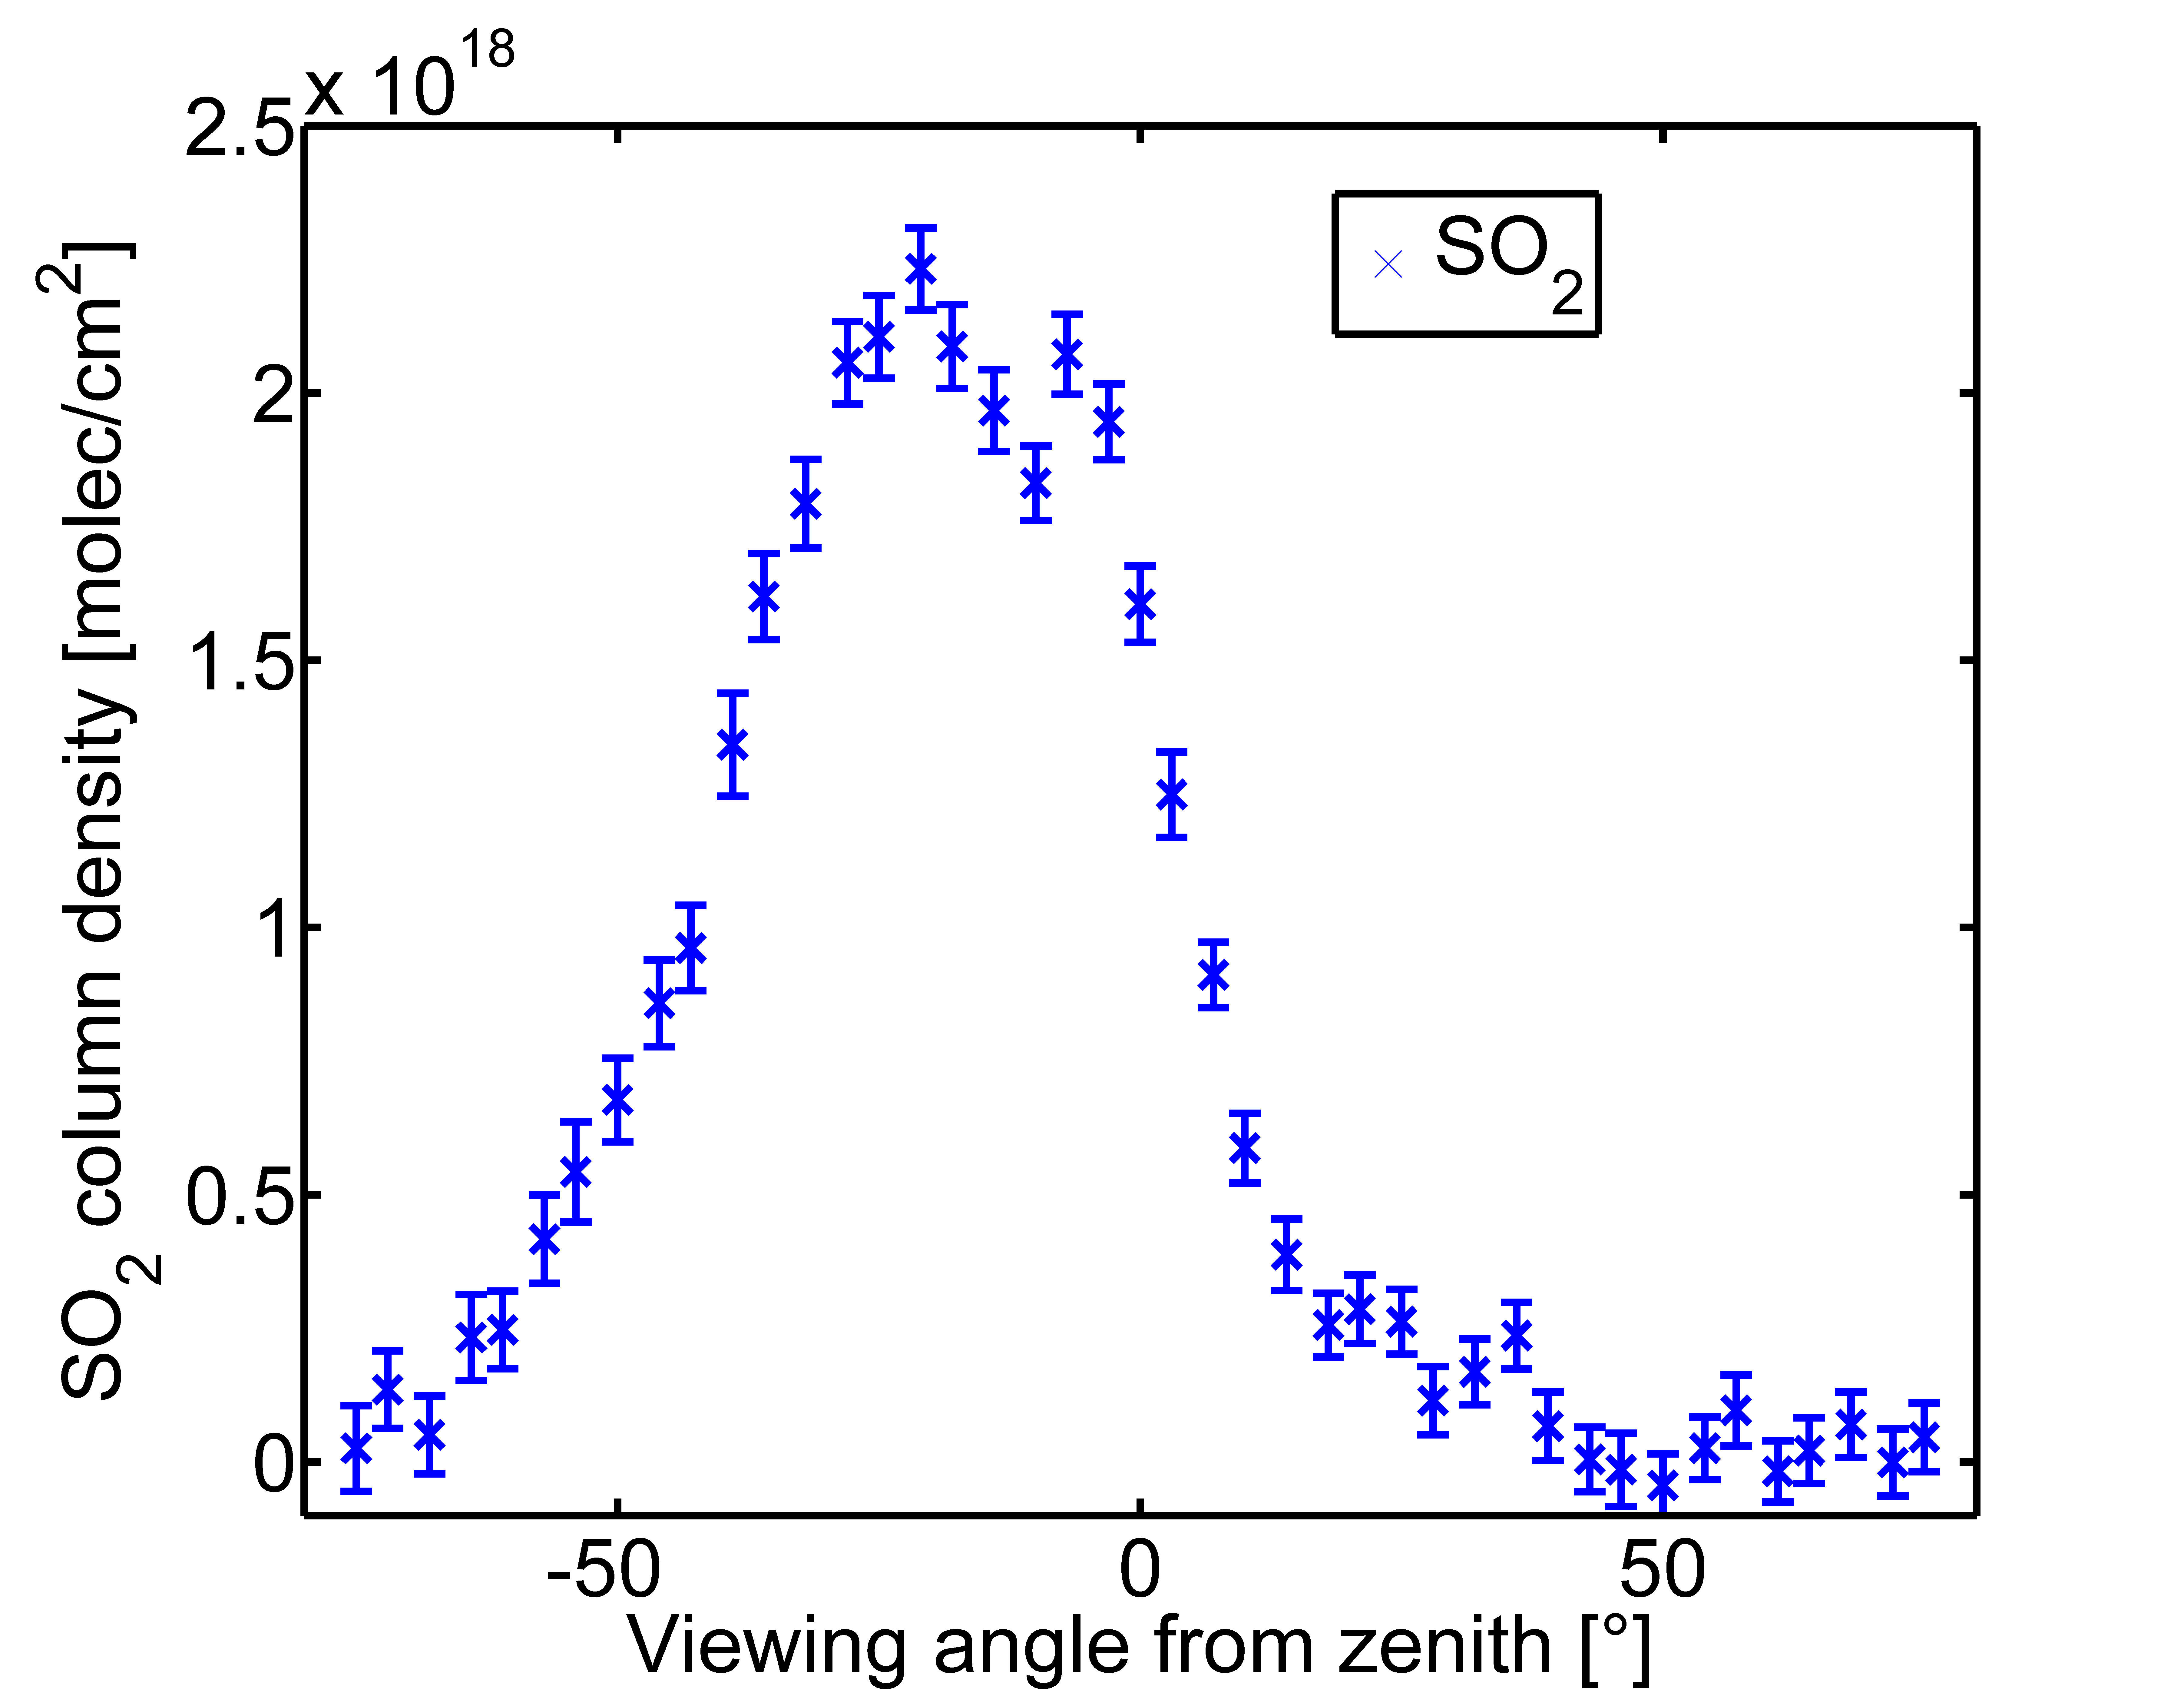
\includegraphics[width=0.51\textwidth]{Bilder/Simon/Bilder_Tung/SO2_Scan_0}}
	\subfigure[]{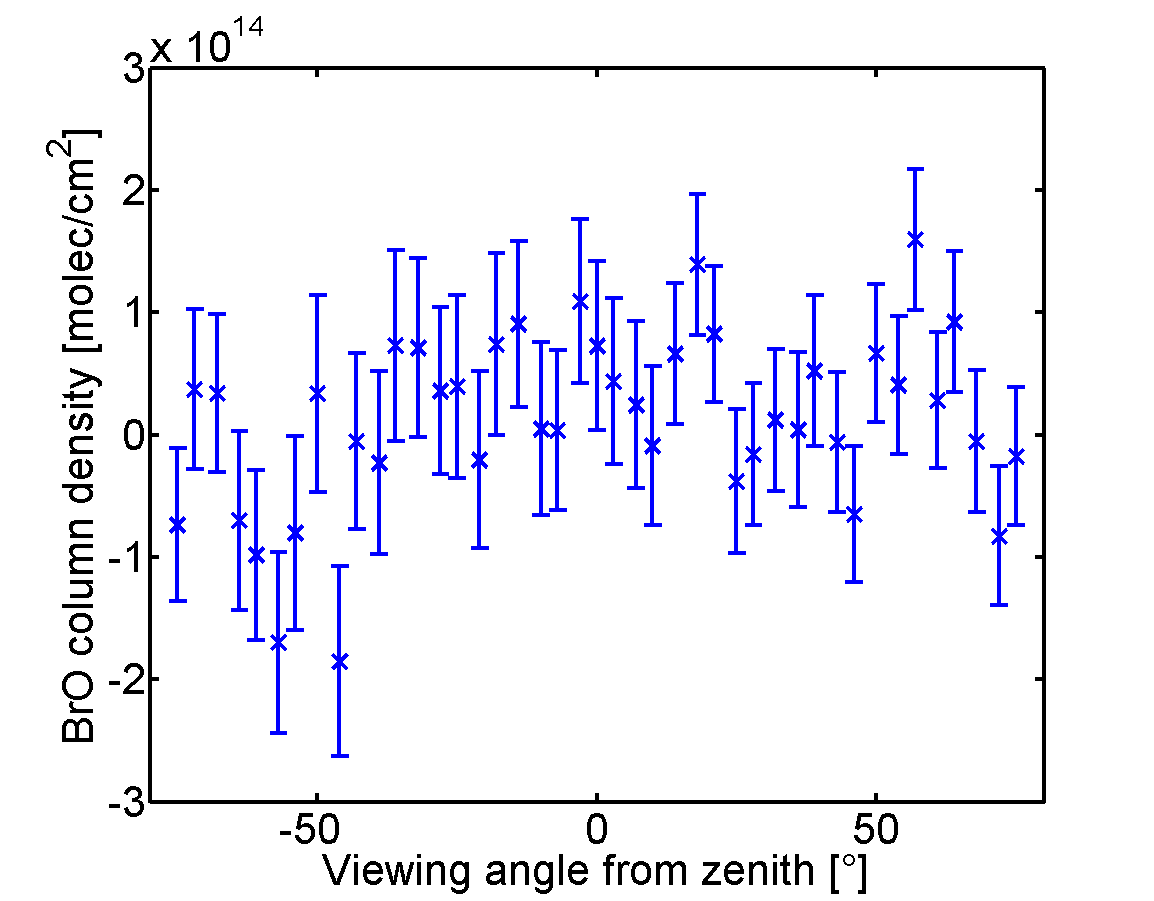
\includegraphics[width=0.51\textwidth]{Bilder/Simon/Bilder_Tung/BrO_Scan}}
	\caption{(a) \ce{SO2} SCD as a function of the elevation angle with error bars computed by the DOASIS fitting routin. (b) \ce{BrO} SCD as a function of the elevation angle with error bars computed by the DOASIS fitting routine.  Taken from \cite{WarnachSimon}}
	\label{fig:plumeref}
\end{figure}
%
In the following we describe the technical implementation of the DOAS approach using the data of NOVAC instruments:\\
%
The first step is to correct each spectrum of the scan for dark current and offset using the dark spectrum.
The next task is to locate the spectra in and outside of the volcanic plume.
First a "pre-reference" (the spectrum recorded at an elevation angle of  0$^{\circ} $) is used to perform the evaluation of the scan spectra recorded at every elevation angle.
For every spectrum of the scan the \ce{SO2} differential slant column density (dSCD) with respect to the pre-reference is calculated using \Cref{eq:F} by the DOASIS fit routine.

The result is \ce{SO2} dSCDs as a function of the elevation angle. This way the elevation angle corresponding to the maximum and the minimum of the \ce{SO2} column density can be determined. The location of the \ce{SO2} maximum defines the location of the plume. The assumption is that the minimum of the \ce{SO2} curve corresponds to a region outside of the plume which is true in most cases. The background \ce{SO2} amount in the earth atmosphere around Tungurahua is usually negligible (see  \Cref{chap:so2}) so we take it as a region of zero \ce{SO2}. \\
We use a gauss fit of the \ce{SO2}-elevation-angle-curve to define the plume region.
%
\begin{figure}
	\centering
	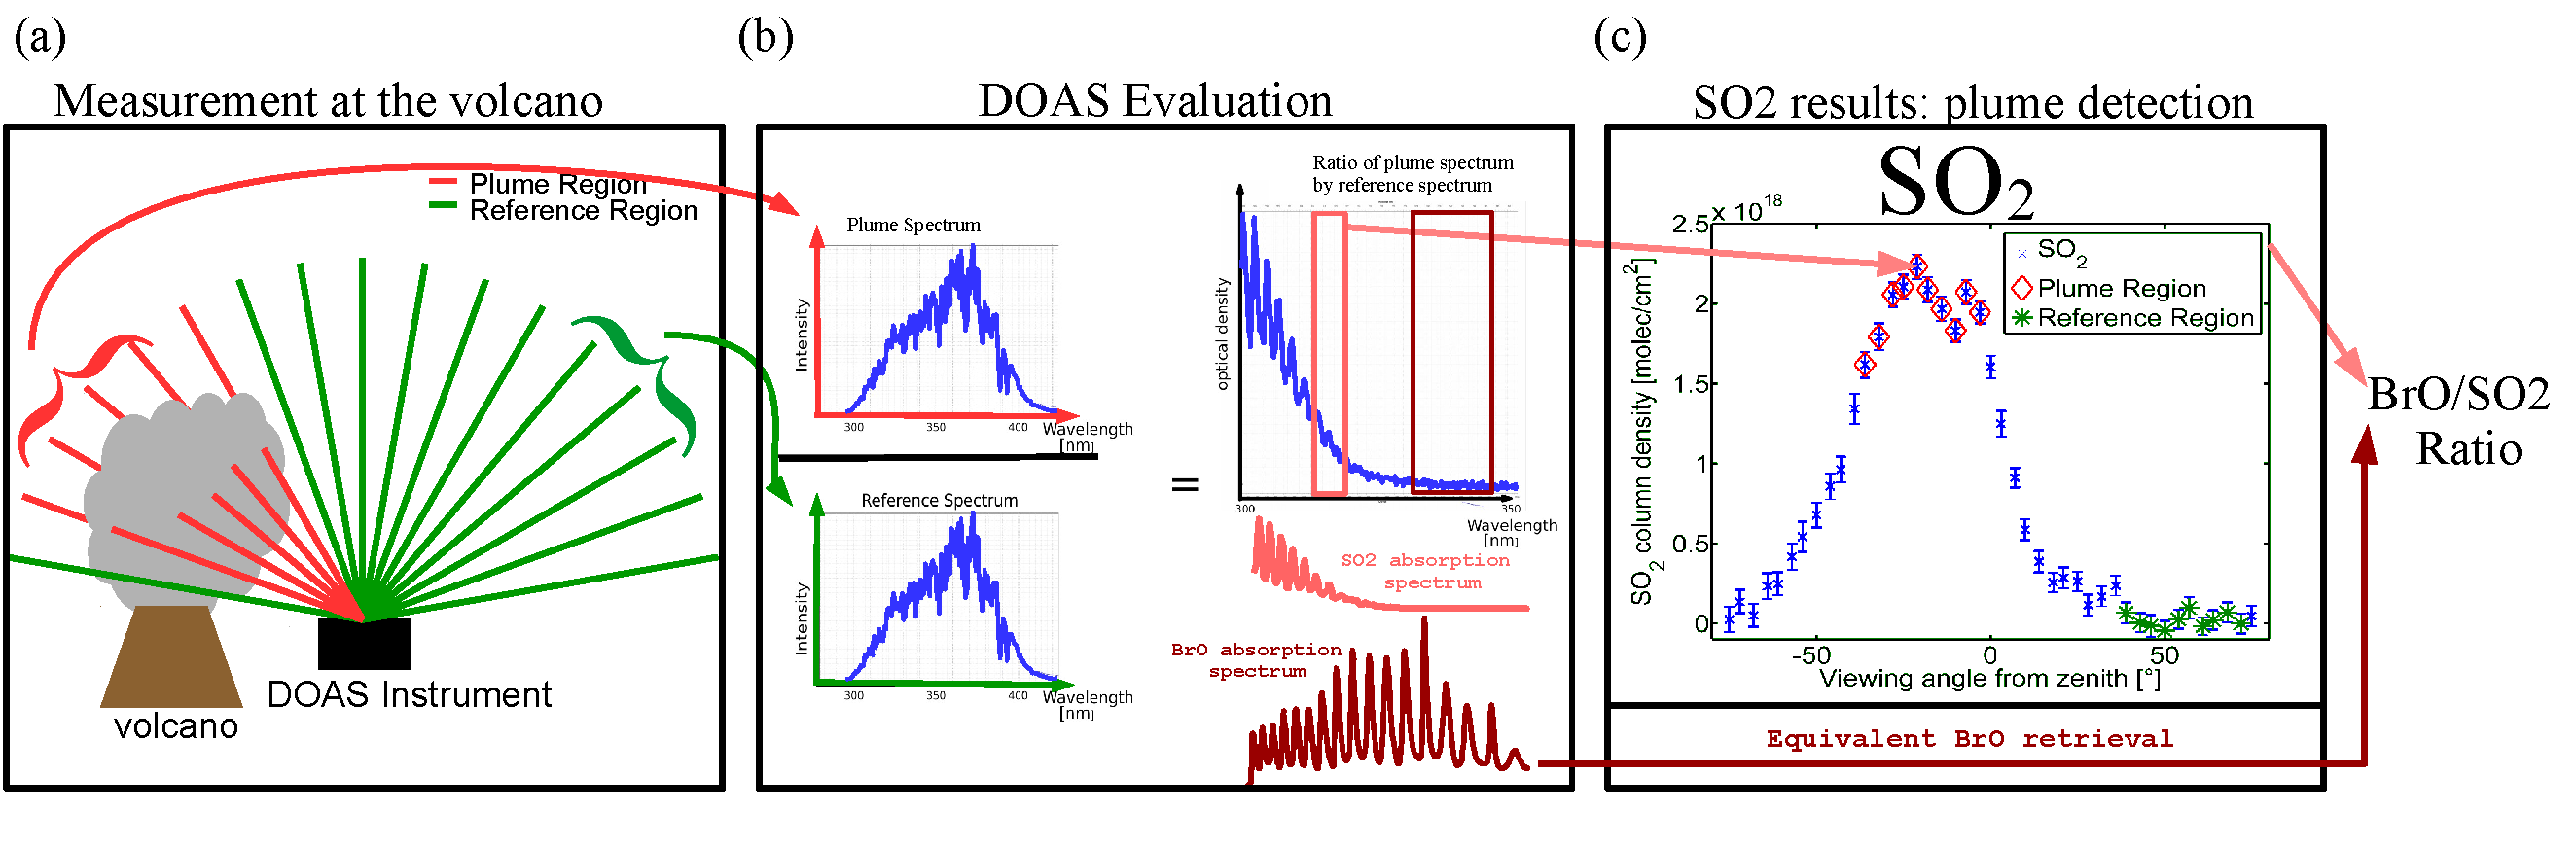
\includegraphics[width=1\linewidth]{Bilder/NOVAC_Eval}
	\caption{NOVAC Evaluation: (a) Measurement at the volcano (b) Evaluation of the spectral data with the DOAS routine using the absorption cross sections of \ce{BrO}  and \ce{SO2}. (c) Finding the location of the plume and reference (taken from \cite{WarnachSimon}) (d) Computation of the ratios BrO/\ce{SO2}}
	\label{fig:NOVAC_Eval}
\end{figure}
The sum over all plume spectra is taken, which are in the elevation angle interval of the gauss peak plus minus one sigma, to increase the photon statistic and to reduce the residuum. If the gauss curve is too wide, what this means in specific is that more then 10 spectra are added within the gauss evaluation, The running mean is calculated and the 10 spectra with the highest \ce{SO2} amount are used for the retrieval. As reference we use the sum of the 10 spectra with the lowest \ce{SO2} amount.\\
The absolute slant column densities (SCD's) of \ce{BrO}  and \ce{SO2} can now be calculated with the previously defined reference and plume spectrum.
In \Cref{fig:plumeref} (a) an example \ce{SO2} SCD as a function of the elevation angle is shown. The \ce{SO2} curve has a maximum at the position of the plume at an elevation angle of approximately $-30^{\circ}$ to $0^{\circ}$  and a reference region at an elevation angle of $40^{\circ}$ to $70^{\circ}$. \Cref{fig:plumeref} (b)  illustrates that  extrema of the \ce{BrO}  curve are not as distinct as it is the case for the \ce{SO2} curve.\\
Since the \ce{BrO} column density is much lower than the \ce{SO2} column density, and just lies slightly above the detection limit, the plume is hard to detect using the \ce{BrO} column density as it is shown in fig. \ref{fig:plumeref} (b). 
Therefore we evaluate BrO only in the plume location determined by using \ce{SO2}.\\
To avoid a distortion of the data as a consequence of relatively bad scans, only scans with a $\chi^2$ (BrO fit) below $10^{-3}$ ($\approx$	95 \% of all suitable scans) are considered.
In a further step multiple reference and plume spectra of successive measurements are added to further increase the fit quality.
\Cref{fig:NOVAC_Eval} visualizes the different steps described above in the retrieval of the BrO/\ce{SO2} ratios.\\
\Cref{fig:algorithm} (b) shows the routine of adding multiple spectra of consecutive measuring times. In the following the spectra resulting from the multi adding technique will be referred to as "Multi Add Spectra". The algorithm for co-adding is visualized in \Cref{fig:algorithm} (b) was invented by \citet{vogel2011volcanic} and \citet{lubcke2014bro}. At Tungurahua periods with significant degassing have a mean temporal resolution of 19 and up to 45 "Multi Add Spectra" per day (resulting from three instruments)\\

The mean standard deviation is about $2.6\cdot10^{13} \frac{molec}{cm^{2}}$. Hereby the standard deviation is estimated as 2 times the DOAS fit error of the multi-scan BrO fit \citet{Stutz:96} \\

The SO2	detection limit is in the order of $6\cdot10^{16}\frac{molec}{cm^{2}}$.\\
%
Taking the \ce{BrO}/\ce{SO2} molar ratios if the column densities are close to zero yields unpredictable and unrealistic results. 
Thus, spectra measured in a thin volcano plume need to be excluded.
This could be achieved by setting a \ce{BrO} or/and an \ce{SO2} threshold. A reasonable \ce{BrO} threshold needs to be at least in the order of the DOAS fit error. The BrO detection limit can be enhanced by an daily averaging, then we get an detection limit of: BrO$_{DT}=\frac{2.6\cdot10^{13}}{n}\cdot\frac{molec}{cm^{2}}$ (n: number of Multi Add Scans per day): However most BrO SCDs are below the detection limit.\\
However rejecting all BrO SCDs below the detection limit leads to an drastical decreases of data points and to systematic elevated \ce{BrO}/\ce{SO2} ratios  \citep{lubcke2014bro}.\\

%
\begin{figure}
	\subfigure[ ]{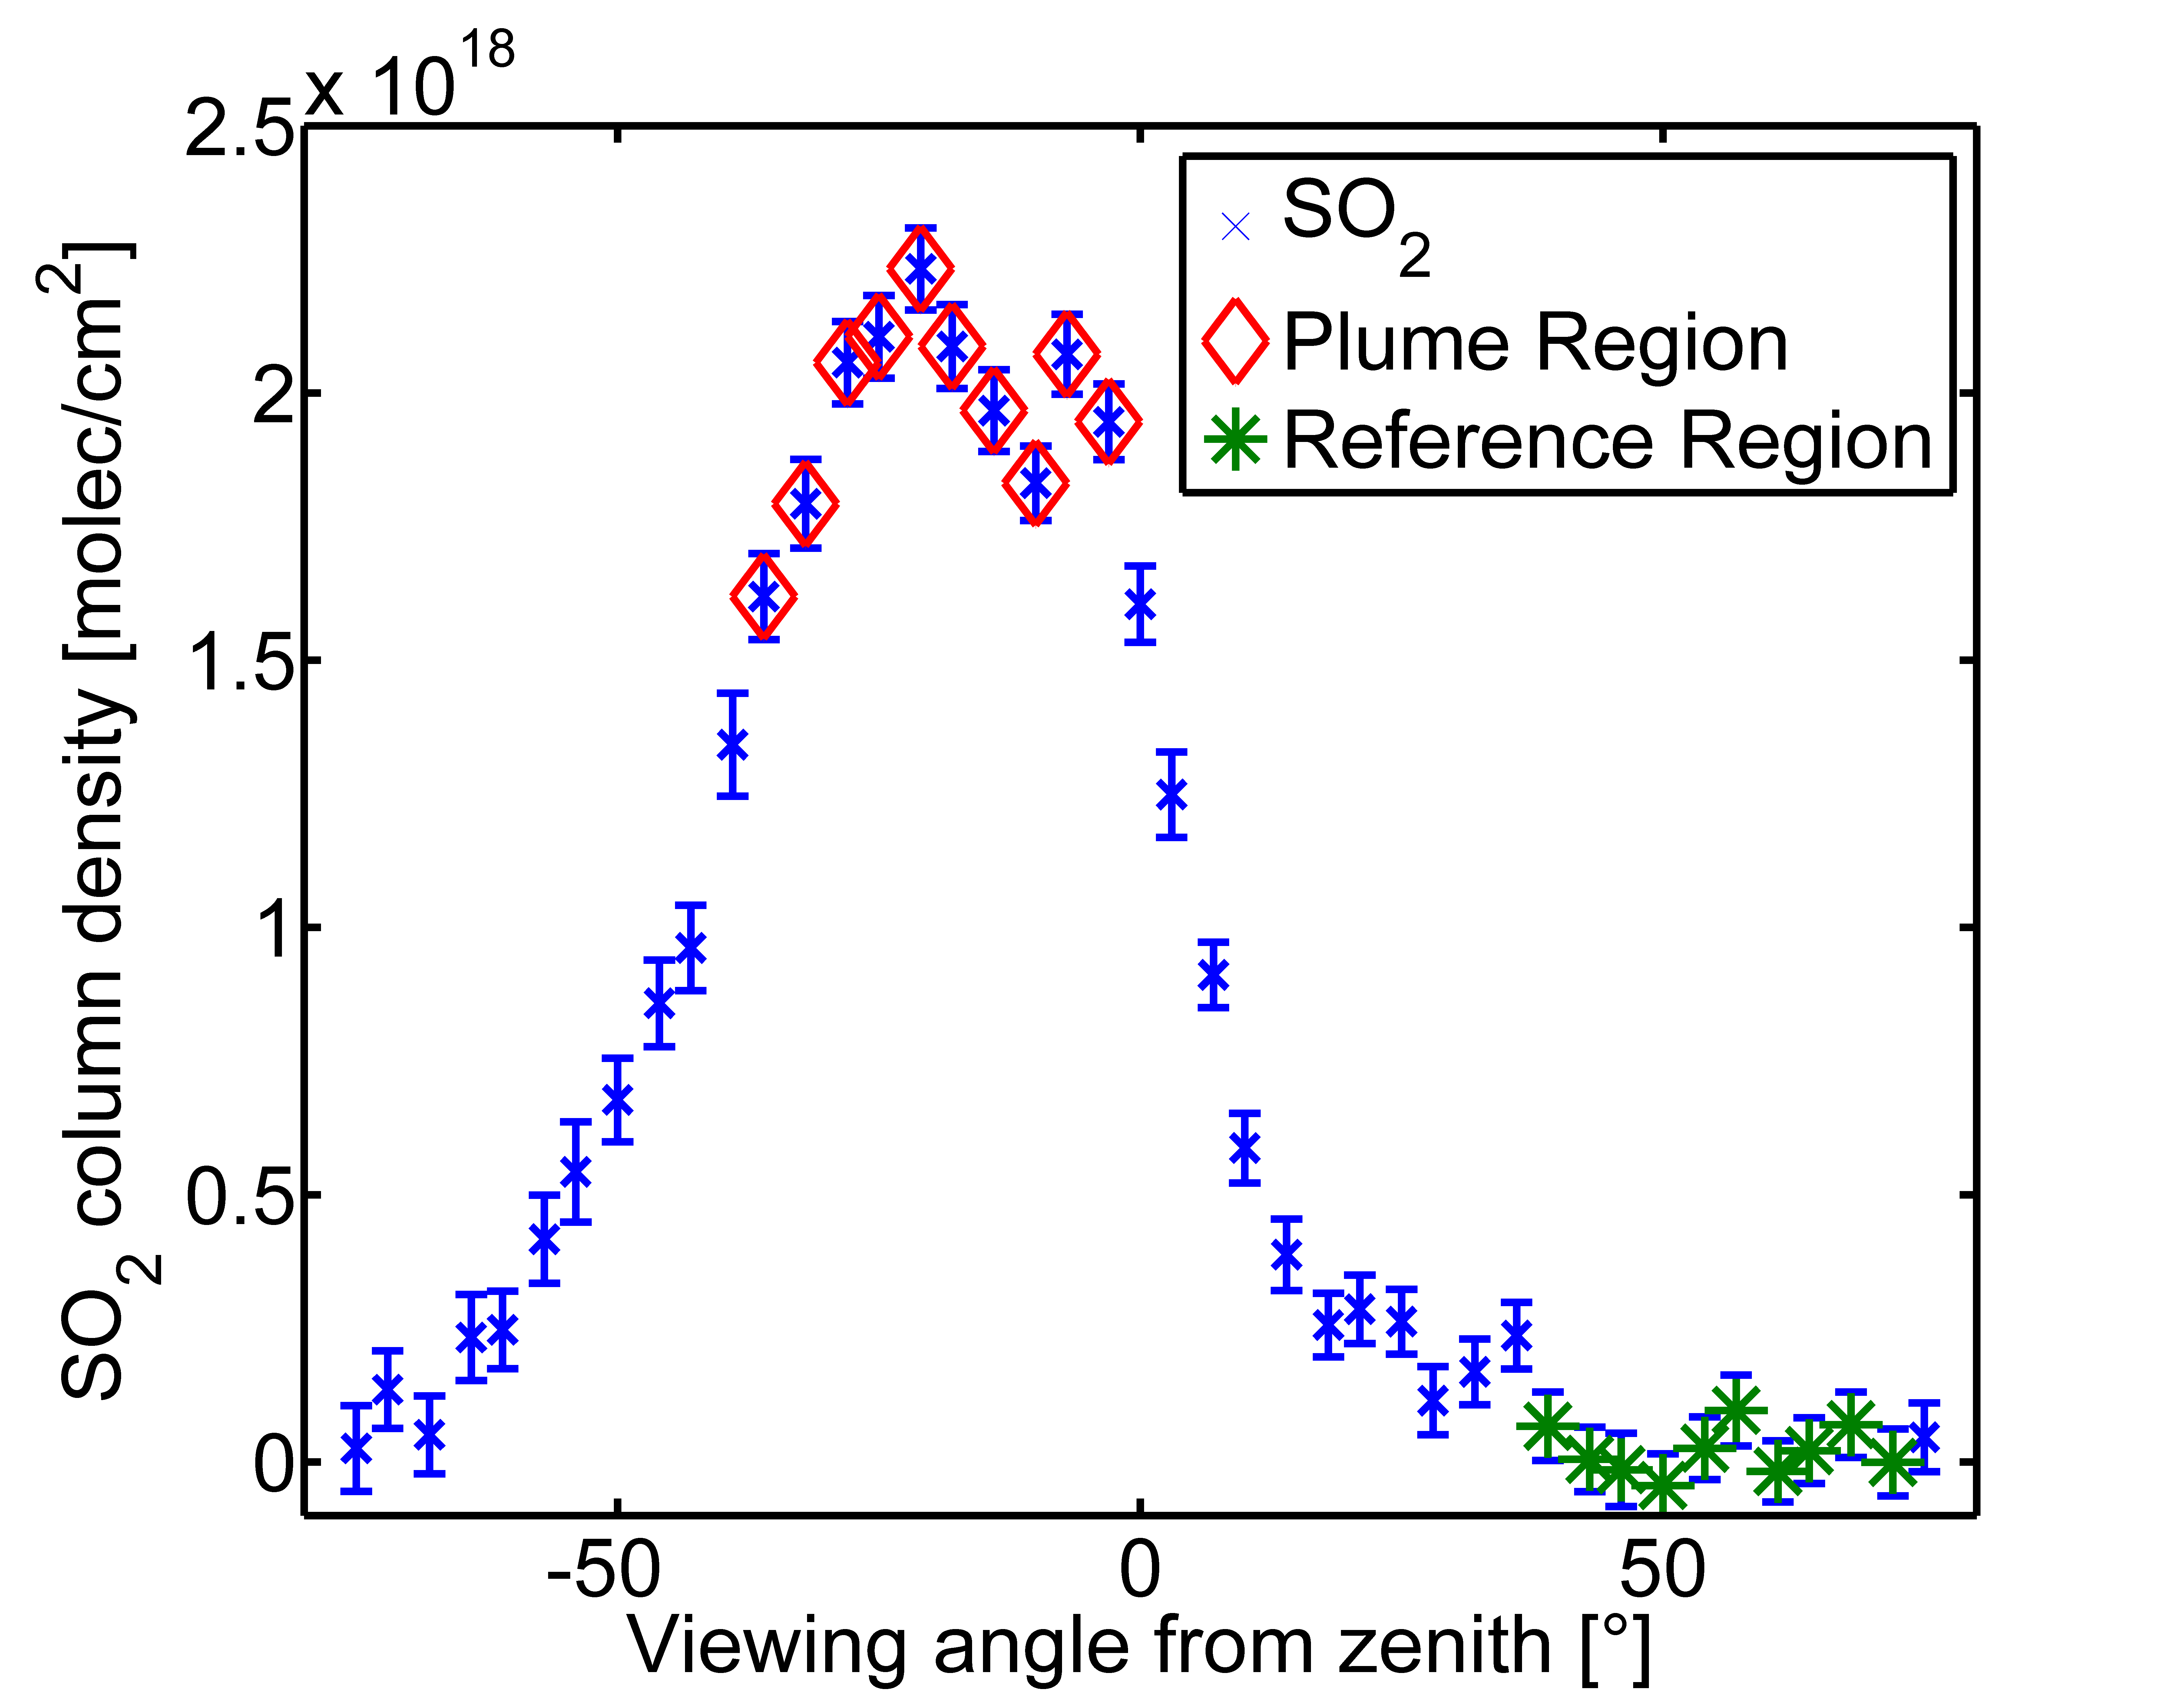
\includegraphics[width=0.53\textwidth]{Bilder/Simon/Bilder_Tung/SO2_Scan}}
	\subfigure[ ]{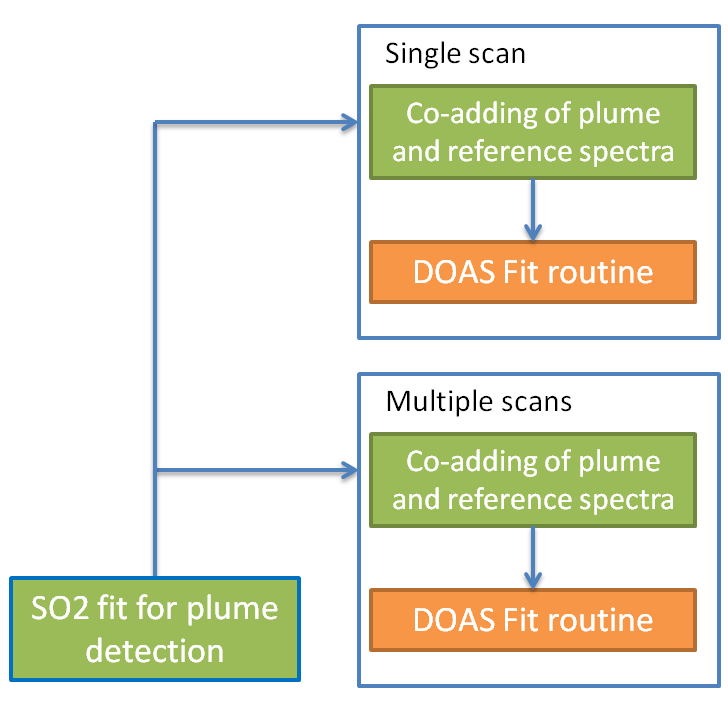
\includegraphics[width=0.47\textwidth]{Bilder/Simon/Bilder_Tung/Algorithm}}
	\caption{(a) \ce{SO2} SCD as a function of the elevation angle. The co-added plume region is marked with red diamonds, and the co added reference region with green stars. From \cite{WarnachSimon}. (b) Flow chart of the \ce{BrO}  and \ce{SO2} evaluation. From \cite{lubcke2014optical}.}
	\label{fig:algorithm}
\end{figure}
The other possibility is to set an \ce{SO2} threshold to ensure only measuring in strong degassing periods. In this thesis an \ce{SO2} threshold (plume limit) of $7\cdot 10^{17} \frac{molec}{cm^2}$ is used for the selection of spectra for the evaluation of the \ce{BrO}/\ce{SO2} ratio. 

Within the data above a SO2 plume limit of $7\cdot 10^{17} \frac{molec}{cm^2}$ the maximum detection limit of the BrO/SO2 ratio is estimated as $(BrO/SO2)_{DT}	=	\frac{\ce{BrO}_{DT}}{SO2_{thres}}=\frac{4	}{\sqrt{n}}\cdot10^{-5}	 \leq 	1\cdot10^{-5}$.
$7\cdot 10^{17} \frac{molec}{cm^2}$ is a high threshold for the column density. However, this approach assures that only strongly significant gas amounts are accounted \citep{lubcke2014bro}. Choosing the \ce{SO2} threshold in this way is a compromise getween a low BrO/SO2 detection limit and a sufficient amount of data.\\

Increasing a plume limit leads to a decrease of usable data. The amount of usable  daily means as a function of the plume limit is shown in \Cref{fig:percentageminso2}. A plume limit of 7$\cdot10^{17}$ leads to a ratio of usable data of approximately 10\%.
\begin{figure}
	\centering
	\subfigure{	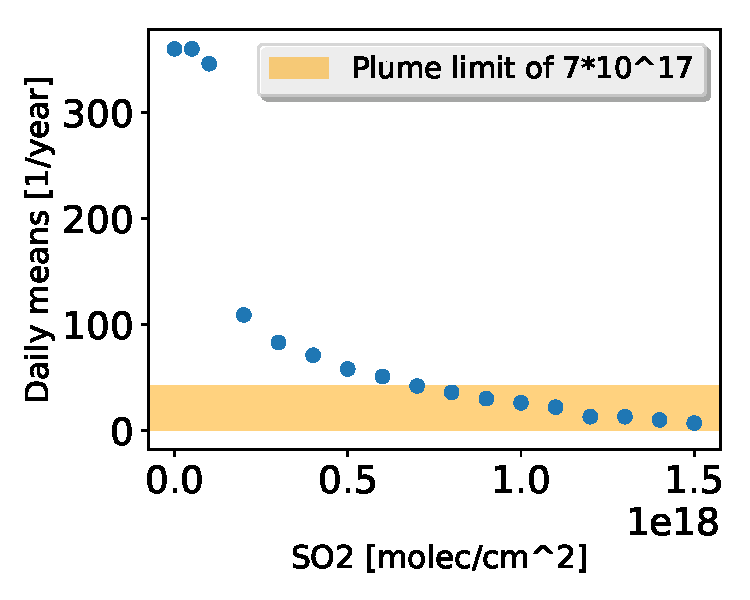
\includegraphics[width=0.49\linewidth]{Bilder/tungpercentage_minSO2}}
	\subfigure{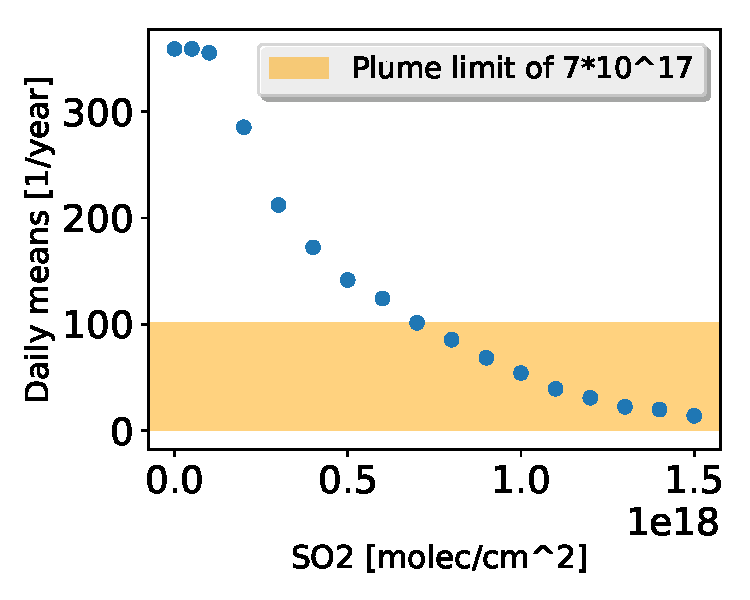
\includegraphics[width=0.49\linewidth]{Bilder/percentage_minSO2}}
	\caption{The decrease of the amount of daily means amount above the plume limit as a function of the SO2 column density. The SO2 SCDs below the actual plume limit of 7$\cdot10^{17}$ are marked with a yellow shade. Left: Data of three instruments at Tungurahua. Right: data of two instruments at Nevado del Ruiz.}
	\label{fig:percentageminso2}
\end{figure}

\section{Contamination problem\label{Chap:Cont}}
The conventional Evaluation is based on the assumption, that the reference is free of volcanic gases. This assumption was checked by using a volcanic gas free a high resolution solar atlas spectrum (see below) to evaluate the reference \cite{lubcke2014}; \cite{salerno2009novel}. In some reference spectra an amount of \ce{SO2}  different from zero is found. Thus we can conclude, that there are some references which contain a non-negligible amount of volcanic trace gases.
In rare (ca. 10\% of the data) scenarios, the
volcanic plume covers the whole scan region.
This could happen if for example the volcanic plume of the day before extends over the hole scan area as a consequence of windless conditions.
In consequence, the reference	is contaminated with volcanic trace gases. Thus, the gas amount is underestimated by the NOVAC-evaluation: In \Cref{fig:contaminated} we see an example from April 2011 (Tungurahua) where the reference region is contaminated by volcanic trace gases. The blue \ce{SO2} curve shows the calculations with the NOVAC-evaluation, but since there is still \ce{SO2} in the reference region, the assumption, that the \ce{SO2} amount could be set to zero in the reference region is wrong. The red curve shows the real \ce{SO2} curve, which lies significantly above the NOVAC -curve.\\
\\	
%
\\
\begin{figure}
	\centering
	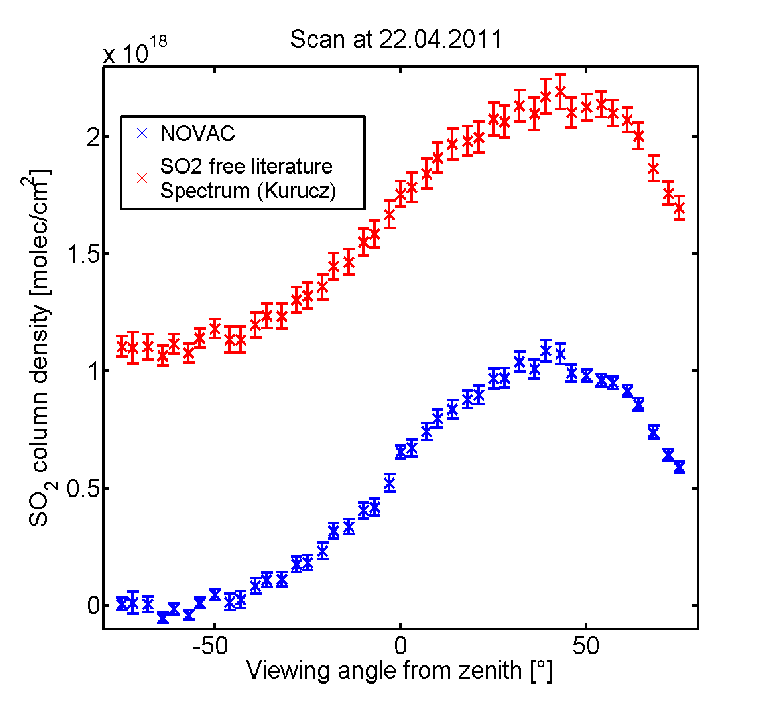
\includegraphics[width=0.7\linewidth]{Bilder/contaminated}
	\caption{Scan with a contaminated reference spectrum from April 2011. From \cite{WarnachSimon}}
	\label{fig:contaminated}
\end{figure}
If the reference region for any reason is
contaminated by volcanic trace gases, there are two possibilities: excluding the contaminated data from the evaluation or the reference spectrum has to be
replaced by a volcanic-gas-free reference. Alternative spectra are a
theoretical solar atlas spectrum or a volcanic-gas-free reference
spectrum recorded by the same instrument at another time.\\
A further possibility is to assume, that contamination only occurs for SO2, but not for BrO due to the smaller lifetimes of BrO, thus it is possible to use the Solar atlas spectrum for the \ce{SO2} evaluation, but the reference, recorded by the NOVAC-instrument at the same time for the BrO retrieval. Hereby the assumption, that BrO is not contaminated need to be proved. \\
%
\\
%
In the following we will discuss the two alternative reference spectra.
%
\subsection*{Evaluation using a Solar Atlas spectrum \label{kuruz}}
An alternative for choosing the region with the lowest column density as reference region is to use a theoretical high resolution solar atlas spectrum as reference \citep{chance2010improved}.
The use of a theoretical solar atlas spectrum as a reference which is completely volcanic-trace-gases-free was first proposed by \cite{salerno2009novel} and evolved by \citep{lubcke2014bro}.
The advantage of using a solar atlas spectrum as reference is, that we know that it is not affected by past or current volcanic gas emissions. Thus, it allows for a retrieval of the absolute trace gas SCDs in the volcanic gas plume. The disadvantage is, that using a solar atlas spectrum comes along with a drawback of precision: The spectral resolution of the theoretical solar atlas spectrum is much  higher than of the NOVAC instruments. Therefore the instrument functions would need to be perfectly modeled and added to the retrieval. This is not straight forward, because the instrumental line-shape varies over the wavelength region and is also mathmatically often not perfectly described by a simple approach like Gauss, lorents,..etc.\\ 
The reduction of precision is acceptable for the
\ce{SO2} retrieval but not suitable for a \ce{BrO} retrieval because then most data would be below the detection limit.\\
%
\\
%
Possible contaminations can be checked
by a theoretical solar atlas spectrum to evaluate the \ce{SO2} amount in the reference.\\

%
\subsection*{Evaluation using a spectrum of the same instrument}
An alternative reference spectrum could be a volcanic-gas-free reference
spectrum recorded by the same instrument at a different time. When using such a reference several problems occur:\\
As described in \Cref{NOVAC} the instruments used in NOVAC do not include features like temperature stabilization. Due to that the measurements are not independent of external parameters. 
So we need to choose a reference recorded at similar conditions with respect to meteorology and	radiation as well as in the temporal proximity due to instrumental changes with time and ambient conditions. Ideally the external conditions should be equal to the conditions at the time when the plume was recorded.\\
\\
%
When performing the evaluation with the Solar Atlas Spectrum as reference, finding the instrument function occur to be a central challenge. If the instrument function for the solar atlas spectrum is found the functions is typically used for a few years This could lead to higher errors due to an gradual worse matching instrument function.
Using the reference of the same instrument but recorded at another day, leads also to problems caused by different instrument functions, but compared to the calculated instrument function used for the evaluation with the solar atlas spectrum those differences in the instrument function could be smaller.
\\
In this work we combine both options in order to
achieve both, enhanced accuracy but still maximum possible precision of
the \ce{SO2} and \ce{BrO} retrievals. So we use the solar atlas spectrum to check for 
contamination and a reference spectrum recorded in temporal proximity by the same instrument as reference.\\
\\
If contamination occurs it is possible to choose a new reference from a list of gas free alternative references. In theory, for ideal instruments all references should lead to
	the same results for the gas retrievals. But instruments are imperfect (see Chapter
	4) thus the reference need to be chosen carefully in order to ensure reliable results.\\
%
\\
As discussed above it might occur, that the reference is contaminated for example by the plume of the day before.
%\textcolor{green}{das verstehe ich jetzt nicht - ich meine wenn wir jetzt das solar atlas spectrum nehmen ueberschaetzen wir ja , weil wir fahne von gestern und heute als eine einzige Fahne zusammen addieren...
%	unterschaetzung haben wir wenn der bei zum beispiel kleiner windgeschwindigkeit -> breite fahne das instrument in keiner richtung fahnen freien himmel sieht - oder bei hoher windgeschwindigkeit und instrument nah am berg die fahne so runtergedreuckt wird das das instrument in der fahne steht..: Florian : @ Nicole zur Überschätzung: wenn wir annehmen, dass die alte, bodennahe Fahne überall die gleiche Dicke hat und die neue Fahne eher im Zenit steht, dann ist der Anteil der alten Fahne zum neuen Gesamtsignal kleiner als der alten Fahne zum neuen Referenzsignal. D.h. Überschätzung ja, aber weniger als simple Addition.} 
If that happens, we underestimate the gas amount by using a contaminated reference. But another possibility is, that the plume itself is also contaminated. This might be the case if the volcanic gas of the volcano is not taken away by the wind, but accumulates at the instrument. If this is the case, using an other reference would lead to an overestimation of the column density of gases. With the data retrieved by the NOVAC instruments it is very difficult to discover whether the plume is contaminated or not. \\

If the contamination is a result of strong emissions of the day before, a dependency of the strength of contamination on the emission of the day before could appear. 
The mean SO2 SCDs of a day (daily mean) could be used as a proxy for the total emission. The strength of contamination can be calculated as the difference between the evaluation for \ce{SO2} with a contaminated reference recorded at the same time as the plume spectrum was recorded and using a gas free reference. Such a plot is shown for Tungurahua and Nevado del Ruiz in \Cref{fig:contaminationdependencyso2}. Even though both plots show a slight increase of contamination strength with the mean amount of \ce{SO2} of the day before, the increase is not significant. Another possible proxy for the SO2 emission would be the maximum SO2 SCD of the day before contamination occures. However, taking the maximum does not lead to more significant relation between the emission and the strength of contamination. \\
Thus the SO2 emission is if it influences the possibility of contamination not the only significant factor. To further examine the reasons for contamination the wind conditions should be studied in particular. 
\textcolor{red}{hier waere es gut noch andere parameter zu testen - wie in Luebcke et al, zum beispile als funktion von Wind geschwindigkeit,..   Für NdR kann ich die Meteorologischen Daten ab 2014 beisteuern.}
\\
However this thesis is build on the assumption, that the plume is free of additional contamination \textcolor{yellow}{Nicole hat hier noch fragen, was ?}. In the following we discuss how to automatically determine an optimal reference from another scan.
\begin{figure}
	\subfigure{
	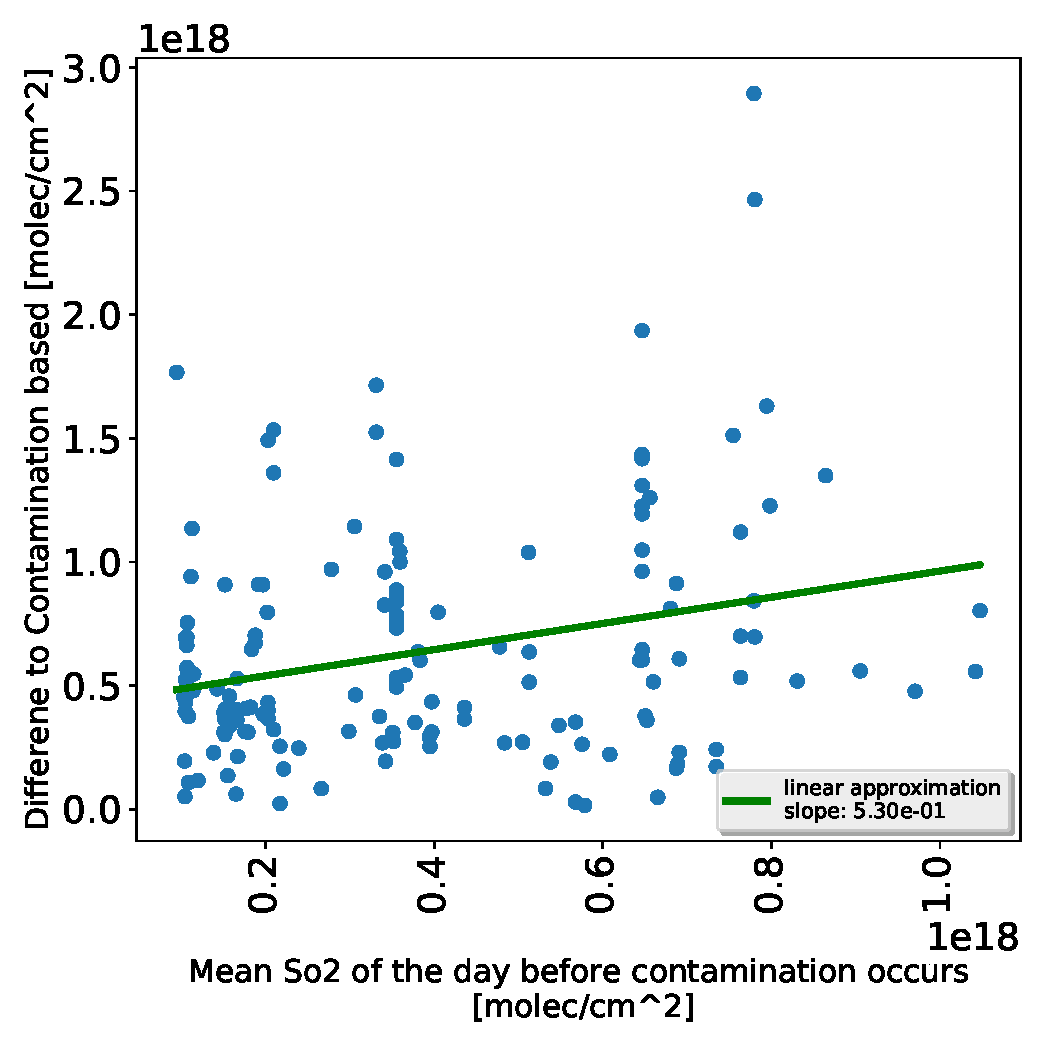
\includegraphics[width=0.5\linewidth]{Bilder/contaminationdependency_so2}}
\subfigure{
	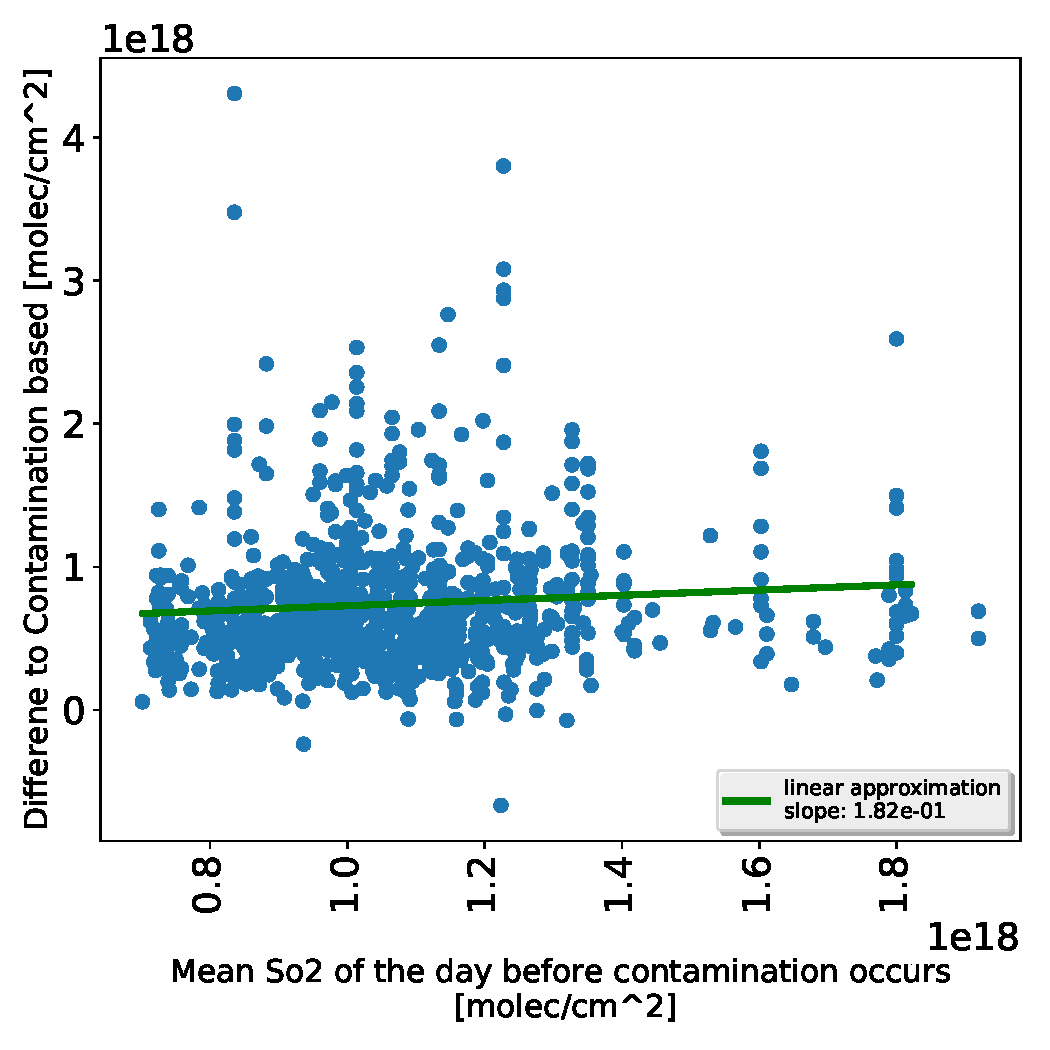
\includegraphics[width=0.5\linewidth]{Bilder/contaminationdependency_so2_Nevad}}
	\caption{The strength of contamination as function of the mean \ce{SO2} column density (daily mean) of the day before. The strength of contamination is defined as the difference in \ce{SO2} SCD  when evaluation with an alternative reference, or neglect the contamination. Left: data from Tungurahua. Right: data from Nevado Del Ruiz. }
	\label{fig:contaminationdependencyso2}
\end{figure}